% documentclass
% set font size=11 (11pt)
% set paper format=A4 (a4paper)
% set equation alignment to left (fleqn)
\documentclass[11pt,a4paper,fleqn]{article}


% Preamble
% to write next to images
\usepackage{graphicx,wrapfig,lipsum}
% use the inputenc and fontenc packages to use French accents
\usepackage[utf8]{inputenc}
\usepackage[T1]{fontenc}
% for pseudocolor
\usepackage{algorithm,algpseudocode}
% for code samples
\usepackage{listings}
% for links
\usepackage{hyperref}
% for color
\usepackage{xcolor}
% allow for arbitrary font size
\usepackage{anyfontsize}
% set the font as Time New Roman (the Latex equivalent, at least)
% \usepackage{mathptmx}
% set the size of the document margins using the geometry package
\usepackage[lmargin=0.97in,rmargin=0.97in,tmargin=1.4in,bmargin=1.4in]{geometry}
% turn the color of footnote markers to black
\renewcommand\thefootnote{\textcolor{black}{\arabic{footnote}}}
% suppress indents on footnotes
\usepackage[hang,flushmargin]{footmisc}
% automatically generates colored brackets around references
\usepackage{fncylab} \labelformat{equation}{(#1)}
% for the bibliography
\usepackage{biblatex}
% supress indent on new paragraphs
\setlength{\parindent}{0pt}
% use the amsmath package to include mathematical symbols
\usepackage{amsmath}
% suppress the space between the left margin and the equations (fleqn still leaves some space by default)
\setlength{\mathindent}{0pt}
% create a new environment to left flush the equation with the align environment
\makeatletter
\newenvironment{lflalign}{ \vspace{-3mm}%
  \def\align@preamble{%
    &\strut@
    \setboxz@h{\@lign$\m@th\displaystyle{####}$}%
    \ifmeasuring@\savefieldlength@\fi
    \set@field
    \hfil
    \tabskip\z@skip
    &\setboxz@h{\@lign$\m@th\displaystyle{{}####}$}%
    \ifmeasuring@\savefieldlength@\fi
    \set@field
    \hfil
    \tabskip\alignsep@
  }
  \flalign}
{\endflalign}
\makeatother
% use the ammssymb package to use mathematical symbols
\usepackage{amssymb}
% create new commands for mathematical symbols
\DeclareMathOperator{\N}{\mathbb{N}}
\DeclareMathOperator{\Z}{\mathbb{Z}}
\DeclareMathOperator{\Q}{\mathbb{Q}}
\DeclareMathOperator{\R}{\mathbb{R}}
\DeclareMathOperator{\Pb}{\mathbb{P}}
% declare the cmsy (computer modern symbol) math alphabet to define appropriate fonts for the U and N mathematical symbols
\DeclareMathAlphabet\mathbcal{OMS}{cmsy}{m}{n}
% create new commands for mathematical symbols
\DeclareMathOperator{\E}{\mathbcal{E}}
\DeclareMathOperator{\Ex}{\mathbb{E}}
\DeclareMathOperator{\F}{\mathbcal{F}}
\DeclareMathOperator{\G}{\mathbcal{G}}
\DeclareMathOperator{\M}{\mathbcal{M}}
\DeclareMathOperator{\HH}{\mathbcal{H}}
\DeclareMathOperator{\QQ}{\mathbcal{Q}}
\DeclareMathOperator{\PP}{\mathbcal{P}}
\DeclareMathOperator{\Noo}{\mathbcal{N}}
\DeclareMathOperator{\U}{\mathbcal{U}}
% use the bbm package to be able to use the double stroke 1 for the indicator function
\usepackage{bbm}
\DeclareMathOperator{\ind}{\mathbbmss{1}}
% use the bm package to use bold characters in math mode
\usepackage{bm}
% create a new command for black square bullets
\newcommand{\bs}{\scalebox{0.7}{$\blacksquare$} \hspace{2mm}}
% use the relsize package to be abe to change the size of mathematical symbols
\usepackage{relsize}
% define a new command for in-line small summation
\newcommand{\ssumm}[2]{\underset{\scriptscriptstyle #1}{\overset{\scriptscriptstyle #2}{\mathlarger{\mathlarger{\mathlarger{\Sigma}}}}} \hspace{0.5mm}}
% define a new command for in-line small products
\newcommand{\sprod}[2]{\underset{\scriptscriptstyle #1}{\overset{\scriptscriptstyle #2}{\mathlarger{\mathlarger{\mathlarger{\Pi}}}}} \hspace{0.5mm}}
% Use the caption package to customize captions (titles) of tables and graphs
\usepackage[font=small,labelfont=bf]{caption}
% use float package to force figure the be positioned where indicated
\usepackage{float}
% use the graphicx package to be able to resize tables
\usepackage{graphicx}

\usepackage{lipsum}% Used for dummy text.
\definecolor{titlepagecolor}{cmyk}{1,.60,0,.40}
\definecolor{namecolor}{cmyk}{1,.50,0,.10} 

\begin{document}

{\fontsize{30pt}{40pt} \textbf{Explain any rule-based model using game theory}\par}

\vspace{10mm}

Target audience: any people with basic knowledge of what an algorithm is. \\

\hyperref[sec:simple-models-everywhere]{Intro: simple models are everywhere}

\hyperref[sec:illustrative-example]{Illustrative example}

\hyperref[sec:complex-example]{Complex example}

\hyperref[sec:explainability]{Explainability}

\hyperref[sec:intuitive-method]{Intuitive method}

\hyperref[sec:link-with-game-theory]{Link with game theory}

\hyperref[sec:shap-article]{Shap article}

\hyperref[sec:linear-regression]{Linear regression}

\hyperref[sec:weighting]{Weighting}

\hyperref[sec:implementation]{Implementation}

\hyperref[sec:results-simple-example]{Results on simple example}

\hyperref[sec:extension-approximation]{Extension: approximation}

\hyperref[sec:conclusion]{Conclusion}


\section{Simple models are everywhere}

\label{sec:simple-models-everywhere}

With the rise of machine learning complexity, one of the key challenges of any company is to understand well enough the impact of the algorithms that it uses. Although there is a tendency for highly sophisticated algorithms such as neural networks, often times in big industries algorithms based on simple rules are more used than fancy machine learning approaches. Note: in this article we will call "model" a set of algorithms. \textit{Explainability} is the concept that a model can be explained in a way that “makes sense” to a human being at an acceptable level (definition from \href{https://c3.ai/glossary/machine-learning/explainability/}{c3.ai}). \\

\section{Illustrative example}

\label{sec:illustrative-example}

Let's say an online shop wants to target certain clients. More specifically, we'll imagine the company wants to focus on the oldest and wealthiest European clients. Thus, the business department decides to select clients satisfying the following criteria: 

- older than 40 years old \\
- based in Europe \\
- salary higher than 60K \\

\begin{center}
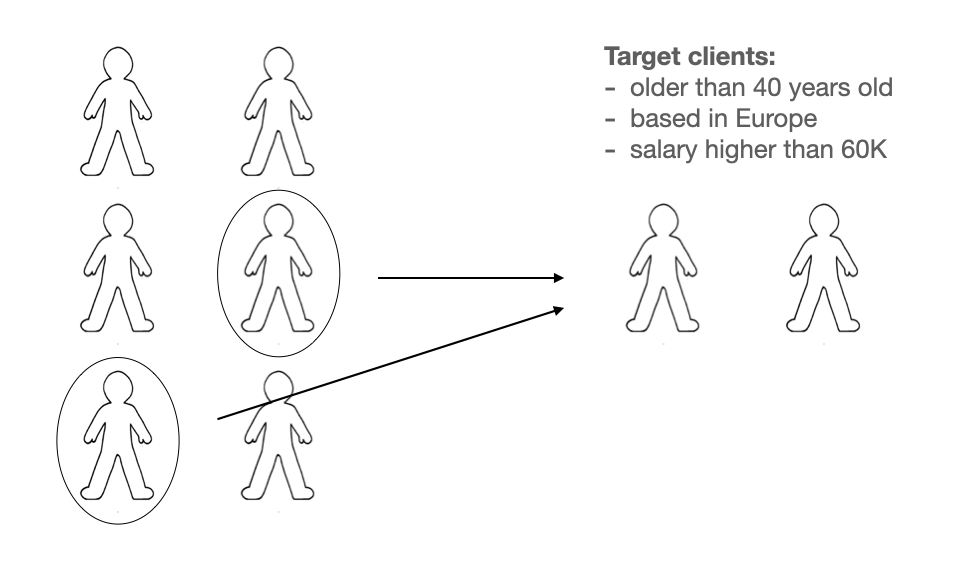
\includegraphics[scale=0.5]{clients-filter.png}
\end{center}

We call those criteria "rules".

\section{Complex examples}

\label{sec:complex-example}

Since there are just a few rules involved here, there is no real need for explainability. But let's say now the business department decides to better target the clients and starts to add more rules:

- older than 40 years old \\
- based in Europe \\
- salary higher than 60K \\
- lives in a house \\
- client since at least 3 years \\
- purchased no more than 10 products \\
- has a least 2 children \\
- bought one swimming suit \\
- had a dog in the past \\
- ...

\section{Explainability}

\label{sec:explainability}

As you can imagine, the possibilities are endless. When using such rules, we may want to know: \textbf{what rules are important here? Which one is really contributing to the selection of clients? Can we rank these rules?} This is exactly what model explainability tries to find out. In other words, it aims at finding what variables are responsible for the result we have. We will present a method that helps answering the question. \\

\section{Intuitive method}

\label{sec:intuitive-method}

Let us use our first illustrative example and assume our client data are composed of age, location and income. The below picture is a summary of our (simplified) database. 

\begin{center}
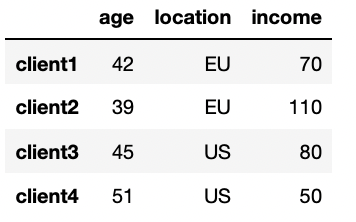
\includegraphics[scale=0.6]{data-simple-example.png}
\end{center}

The used rules are the following:

- rule 1: age>40 \\
- rule 2: location="EU" \\
- rule 3: income>60 \\

Now we want to know what rule is really important here? Which one is the most "selective"? One intuitive way to answer this question is to remove each rule one by one, and see how it changes the results. \\

We note that when using the three rules, we end up with 25\% of clients since only one client is not filtered out. 

When removing only rule 1 (age) we end up with 50\% of the clients. 

When removing only rule 2 (location) we end up with 50\% of the clients.

Thus, our first analysis suggests that rule 1 and rule 2 are equally important. \\

When removing rule 3 (income) we end up with 25\% of the clients.

Thus, our first analysis suggests that rule 3 is not so important since adding it doesn't change the final result. \\

But is this analysis complete? No. \\

To compare the impact of rule 1  and rule 2 we can't just remove these rules one by one since rule 3 and rule 2 both filter out client4. Thus, removing rule 1 or rule 2 doesn't make any difference on the final result (50\% in both cases). Because of this overlapping  effect, we need to look at other combinations. For example, what happen if we use \textit{only} rule 1 or rule 2? With rule 1 only, only one client is filtered out. With rule 2 only, 2 clients are filtered out. \textbf{Unlike our previous conclusion, here rule 2 seems more selective (and thus more important) than rule 1}. \\

To sum up, assessing the rule importance requires us to go over all possible combinations. \\

\section{Link with game theory}

\label{sec:link-with-game-theory}

Now here comes the link with game theory. 
Game theory is a field that consists in analyzing the interactions of individuals (agents) within a society. We typically look at what value an agent brings to the society. This value is called \textit{marginal contribution}. How does it link to our problem? Instead of having individuals as agents, let's say the rules are the agents. We now want to see what contribution each rule brings to the model. \\

Since a rule can be added or removed, the total possible combinations of rules is $2^R$ with $R$ the number of rules in total. We can draw the different combinations in a powerset:

\begin{center}
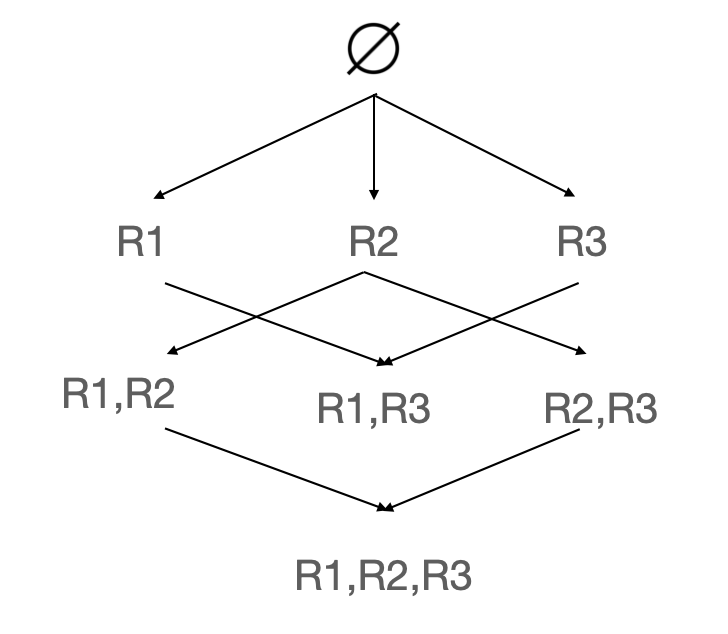
\includegraphics[scale=0.6]{powerset.png}
\end{center}

We can see here that the number of combinations is $2^3 = 8$. \\

\section{Shap article}

\label{sec:shap-article}

The method proposed below is largely inspired by the article "A Unified Approach to Interpreting Model Predictions". The authors show that a way to assess variable importance is to test all combinations and see how each one impact the result. In our use case, the variables (called "feature" in the article) are the \textbf{rules} themselves. The main assumption behind this approach is that the items explaining the model follow a linear relationship:

$$g(z) = \phi_0 + \sum_{i=1}^M \phi_i z_i$$

Let's dive a bit more in the parameters. \\

$g$ is the \textit{explanation} model. It's simply the total effect of the rules on the result.

$z \in \{0,1\}^M$ are all possible combination of rules. $0$ indicates that the rule is removed from the model, $1$ indicates that a rule is added to the model. As an illustration, $(0,1,0)$ is when only rule 2 is used.

$M$ is the number of rules. 

$\phi_i \in \mathbb{R}$ are the Shapley values. The Shapley values reflect the importance of a rule in the model. As an example, if Shapley(rule 1) = 3 and Shapley(rule 2) = 5 it shows that rule 2 contributes more to the model than rule 1. The rationale behind such values are based on some principles that we won't elaborate here but that are well described in the article. \\

\section{Linear regression}

\label{sec:linear-regression}

The equation above shows us that the Shapley values can be found using an OLS method.

$$\phi = (z^Tz)^{-1}z^Ty$$

In our example:

$$z = \begin{pmatrix}
0 & 0 & 0 & 1\\
1 & 0 & 0 & 1\\
0 & 1 & 0 & 1\\
0 & 0 & 1 & 1\\
1 & 1 & 0 & 1\\
1 & 0 & 1 & 1\\
0 & 1 & 1 & 1\\
1 & 1 & 1 & 1
\end{pmatrix}$$

Note: the last column stands for the intercept. It's common practice to use the intercept when the variables are not centered, which is the case here.

$$y = g(z) = \begin{pmatrix}
1 \\
0.75 \\
0.5 \\
0.75 \\
0.25 \\
0.5 \\
0.5 \\
0.25
\end{pmatrix}$$

\section{Weighting}

\label{sec:weighting}

Now a small subtlety. So far, all combinations are weighted the same. But the authors propose to penalize mixed combinations (e.g. [0,0,1,1]) and encourage more "pure" combinations (e.g. [0,1,1,1]). The intuition behind such behaviour is well explained on Christoph Molnar’s website: \\

"We learn most about individual features if we can study their effects in isolation. If a coalition [ndlr combination] consists of a single feature, we can learn about this feature’s isolated main effect on the prediction. If a coalition consists of all but one feature, we can learn about this feature’s total effect (main effect plus feature interactions). If a coalition consists of half the features, we learn little about an individual feature’s contribution, as there are many possible coalitions with half of the features."

The weights are thus defined as such:

$$\omega_{z_i} = \frac{R-1}{C_{|z_i|}^R |z_i|(R-|z_i|)}$$

with $|.|$ being the number of non-zero elements in $z_i$. \\

[Understand formula] \\

The formula may seem complicated. Essentially it is used to have lower weights for mixed combinations as explained above. In our simple example with 3 rules only, the weights are all the same ($1/3$).

\section{Implementation}

\label{sec:implementation}

The implementation of the Shapley values can be found on the \href{https://shap.readthedocs.io/en/latest/example_notebooks/tabular_examples/model_agnostic/Simple%20Kernel%20SHAP.html}{Shap's documentation}. \\

Now we need to create our own "prediction" function. Since we are using rules and not features, if a client satisfies all rules, he is not filtered out and has a probability=1 of being included. \\

We first store the rules we want to assess in a dictionary. The Python function \textit{eval} will be very convenient to test whether a condition is satisfied.

\lstset{language=Python}
\lstset{frame=lines}
\lstset{caption={prediction function}}
\lstset{label={lst:code_direct}}
\lstset{basicstyle=\footnotesize}
\begin{lstlisting}

dict_rules = {
    'rule1':'age>40',
    'rule2':'location=="EU"',
    'rule3':'income>60'
}

def scoring_simul(row, activated_rules):
    rules_res = []
    if activated_rules[0]==1:
        age = row['age']
        rules_res.append(eval(dict_rules['rule1']))
    if activated_rules[1]==1:
        location = row['location']
        rules_res.append(eval(dict_rules['rule2']))
    if activated_rules[2]==1:
        income = row['income']
        rules_res.append(eval(dict_rules['rule3']))
    if False not in rules_res:
        return 1
    return 0

\end{lstlisting}

\section{Results on simple example}

\label{sec:results-simple-example}

The Shapley value computation shows that rule 2 is the most important one. Then comes rule 1 and finally rule 3. We note that all rules contribute negatively to our results. This is expected since adding a rule necessarily filter out more clients.

\begin{center}
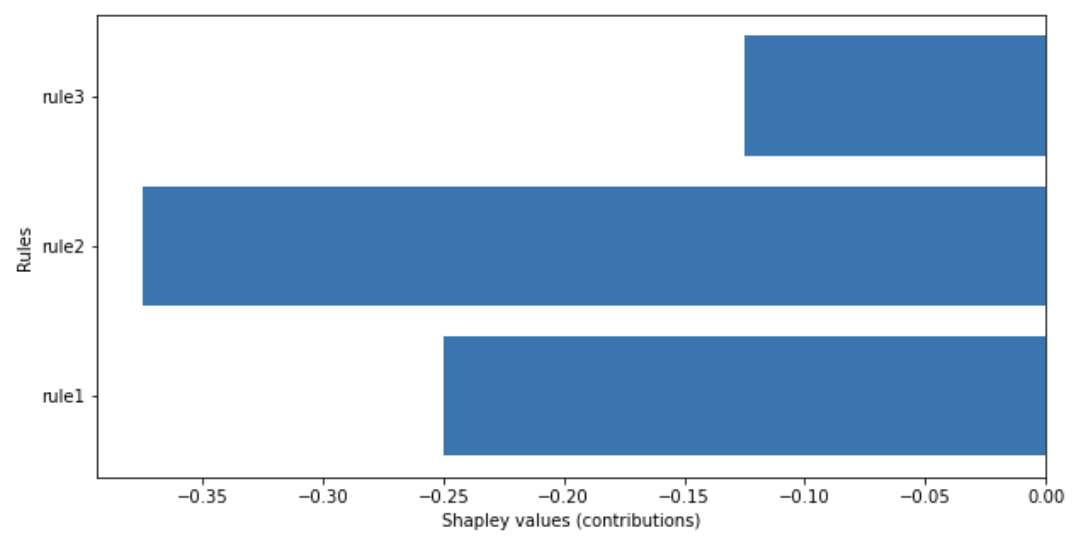
\includegraphics[scale=0.6]{shapley-results.png}
\end{center}

\section{Extension: approximations}

\label{sec:extension-approximation}


\section{Conclusion}

\label{sec:conclusion}

In this article I have presented a method to assess the importance of rules that compose a simple model. I first tried out an intuitive method that is unfortunately incomplete. Then I showed a method based on game theory that consider all possible cases to correctly assess the model. I finally gave some references to go deeper in the understanding of the theory. I hope some materials can be reused for your use case. Feel free to reach out to me via the comment section!


\vspace{10mm}

\end{document} 